% Elsevier CAS double-column template: the layout the journal itself uses,
% with the ARTICLE INFO / ABSTRACT band and ORCID marks beside the authors.
% (Template taken from the authors' PACT manuscript; the original is kept in _template_original/.)
\documentclass[a4paper,fleqn]{cas-dc}

\usepackage[numbers,sort&compress]{natbib}
\usepackage{amsmath,amssymb,amsthm,booktabs,multirow,graphicx,xcolor,float,xspace}
\usepackage{algorithm,algpseudocode}
\usepackage{tikz}
\usetikzlibrary{arrows.meta,positioning,fit,calc}
% Side margins: the class leaves 18 mm each side on a 210 mm page; 15 mm gives
% each column about 3 mm more to work with without crowding the trim.
\setlength{\textwidth}{180mm}
\setlength{\oddsidemargin}{-10.4mm}
\setlength{\evensidemargin}{-10.4mm}

\usepackage{fancyhdr}
\usepackage{microtype}
\emergencystretch=1em
\usepackage{tabularx}
% Weighted, ragged-right X column; the weights in one table sum to its column count.
\newcolumntype{L}[1]{>{\raggedright\arraybackslash\hsize=#1\hsize}X}
% One family throughout: the sans slot is mapped onto the body face.
\renewcommand{\sfdefault}{\rmdefault}
\renewcommand{\ttdefault}{\rmdefault}
\hypersetup{hidelinks}

\graphicspath{{figures/}}
\newcommand{\ERNP}{ERNP\xspace}
\newcommand{\E}{\mathcal{E}}
\newcommand{\R}{\mathbb{R}}
\newtheorem{proposition}{Proposition}
\newtheorem{remark}{Remark}
\newcommand{\friedmanp}{0.079}


\begin{document}

\let\WriteBookmarks\relax
\def\floatpagepagefraction{1}
\def\textpagefraction{.001}

\shorttitle{Adapting NIDS only through trusted evidence}
\shortauthors{A. Vo Le Thien}

\title[mode=title]{Adapting Network Intrusion Detectors Only Through Trusted Evidence:
Evidence-Retracted Novelty Priors for Label-Efficient Zero-Day Detection}

% TODO(authors): add co-authors and their affiliations; keep the corresponding-author mark on the right person.
\author[1]{An~Vo~Le~Thien}
\cormark[1]
\ead{volethienank16@siu.edu.vn}

\affiliation[1]{organization={Faculty of Computer Science, The Sai Gon International University},
                city={Ho Chi Minh City},
                country={Viet Nam}}

\cortext[1]{Corresponding author}

\begin{abstract}
Network intrusion detection systems (NIDS) in production must detect attack families never seen in training, tolerate benign traffic drift, and adapt with the few labels that analysts can provide. Detectors that adapt by absorbing the traffic they accept can be steered by slow poisoning, while continual learners that avoid this depend on hundreds of labels per day. We propose \ERNP (Evidence-Retracted Novelty Prior), a detector whose only adaptation channel is the retraction of a structured novelty prior where analysts have confirmed benign traffic. \ERNP estimates a density ratio between benign evidence and the union of attack evidence and a prior built by partially swapping features between benign flows; unlabelled traffic never enters the model. We prove that retraction is local and bounded by analyst errors, and that detection far from confirmed evidence is preserved up to a computable factor. On four temporally split benchmarks, five seeds and a causal protocol, \ERNP has the best mean rank against five recent detectors (SSF, OWAD, CADE, Trident, MemStream), with mean F1 0.867 against 0.671 for the strongest. With 25 labels per day it outperforms SSF using 200--400, and a counterfactual that feeds \ERNP its own verdicts instead of analyst evidence collapses from 0.74 to 0.07 zero-day payload recall under controlled poisoning. It has the best AUROC and AUPRC on three of the four datasets. On ToN, whose benign traffic changes regime from day to day, it has the best F1 and MCC when the same labels are delivered every 4\,h rather than once a day. \ERNP does not win everywhere: it is on par with CADE on unsampled CIC-IDS2017, and it degrades when analysts mislabel 10\% or more of the queried alert groups.
\end{abstract}

\begin{keywords}
network intrusion detection \sep zero-day attacks \sep concept drift \sep poisoning
\sep active learning \sep density-ratio estimation
\end{keywords}

\maketitle

\pagestyle{fancy}
\fancyhf{}
\fancyhead[L]{\footnotesize A.~Vo Le Thien}
\fancyfoot[C]{\footnotesize\thepage}
\renewcommand{\headrulewidth}{0pt}
\renewcommand{\footrulewidth}{0pt}
\fancypagestyle{plain}{\fancyhf{}\renewcommand{\headrulewidth}{0pt}%
  \renewcommand{\footrulewidth}{0pt}}
\thispagestyle{empty}

%======================================================================
\section{Introduction}
\label{sec:intro}
%======================================================================
A machine-learning NIDS is trained on the traffic of a past period and operates on a stream in which new attack families appear, benign behaviour drifts, and a security operations centre (SOC) can inspect only a small fraction of the alerts \cite{sommer2010outside,arp2022dos}. Three requirements follow. The detector must (i) alert on attack families absent from its training data, (ii) adapt to benign drift so that the false-positive rate (FPR) stays within analyst capacity, and (iii) do both with a small daily labelling budget.

Adaptation is where these requirements collide. Streaming detectors such as MemStream \cite{bhatia2022memstream} and Kitsune \cite{mirsky2018kitsune} update their model of normality with the traffic they accept. This follows benign drift without labels, but it also lets an adversary move the model: traffic that drifts slowly from benign towards malicious is accepted at every step and eventually becomes normal. This ``boiling-frog'' vulnerability has been analysed for centroid and PCA-based detectors \cite{kloft2012security,rubinstein2009antidote}. Label-driven continual learners such as SSF \cite{zhang2025ssf} and OWAD \cite{han2023owad} do not absorb unlabelled traffic in the same way, but they re-train on hundreds of analyst labels per adaptation window. Drift detectors such as CADE \cite{yang2021cade} and open-set classifiers such as Trident \cite{zhao2024trident} rank novel samples well but do not follow benign drift, which appears as a high FPR at a fixed operating point (Section~\ref{sec:rq1}).

This paper starts from a simple observation. A detector that separates benign traffic from an explicit model of \emph{novelty} can adapt in the opposite direction to the usual one. Instead of \emph{enlarging} its model of normality with accepted traffic, it can \emph{shrink} its model of novelty, and only where an analyst has confirmed that the traffic is benign. We call the resulting detector \ERNP (Evidence-Retracted Novelty Prior). \ERNP trains a classifier to separate benign evidence from attack evidence and from a structured novelty prior of synthetic flows obtained by swapping a random subset of features between benign flows. Each day, alerts are grouped and the analyst labels one representative per group. Groups confirmed benign retract the prior mass in their neighbourhood; groups confirmed malicious are added to the attack evidence. The unlabelled stream never enters the model.

We ask five research questions.
\begin{enumerate}
  \item \textbf{RQ1 (zero-day detection):} under a causal protocol with benign drift and equal label budgets, does \ERNP detect unseen attack families better than five recent detectors?
  \item \textbf{RQ2 (poisoning):} when an adversary targets the adaptation process by slow poisoning, is \ERNP more robust than these detectors, and does its robustness come from the trusted-evidence rule?
  \item \textbf{RQ3 (label efficiency):} how many labels per day does \ERNP need compared with label-using detectors?
  \item \textbf{RQ4 (mechanism):} which components produce the performance, and do the stated properties hold on real traffic?
  \item \textbf{RQ5 (deployment):} how sensitive is \ERNP to its hyper-parameters and to analyst errors, and what does it cost?
\end{enumerate}

The contributions are the following.
\begin{enumerate}
  \item \textbf{Adaptation through trusted evidence only.} We formulate NIDS adaptation as the retraction of a novelty prior by analyst-confirmed benign evidence, which makes the detector invariant to the volume and duration of unlabelled traffic. We prove that retraction is local and that its corruption is bounded by the number of analyst errors (Proposition~\ref{prop:p1}), that local false alarms vanish where benign evidence accumulates (Proposition~\ref{prop:p2}), and that detection far from benign evidence is preserved up to a computable factor (Proposition~\ref{prop:p3}).
  \item \textbf{A structured novelty prior} that keeps every benign marginal and breaks cross-feature dependencies. Compared with the uniform negative sampling of Sipple \cite{sipple2020negative} and with a product-of-marginals prior, it raises F1 by 0.26--0.29 on average (Section~\ref{sec:rq4}).
  \item \textbf{A fidelity-checked comparison.} We compare against five recent detectors on four temporally split benchmarks, under a causal protocol and at a common 1\% FPR operating point. The implementations reproduce the published results of CADE and OWAD on the authors' own data. We add each baseline's best configuration, classical references, a classifier-plus-active-labelling ablation, an IP-novelty leakage check and an unsampled-scale check (Sections~\ref{sec:experiments}--\ref{sec:results}).
  \item \textbf{Label efficiency and a causal account of robustness.} \ERNP with 25 labels per day outperforms SSF with 200--400. A counterfactual that replaces analyst evidence by \ERNP's own verdicts isolates the mechanism: under controlled poisoning its zero-day payload recall drops from 0.74 to 0.07. The settings in which \ERNP does not win are reported as results (Section~\ref{sec:discussion}).
\end{enumerate}

The novelty claim is methodological. Classification against a reference distribution and learning from analyst feedback are both known (Section~\ref{sec:related}). The contribution is an adaptation rule in which trusted evidence \emph{retracts} a structured novelty prior. We state its guarantees, measure the conditions under which it holds, and report where it fails.

The remainder of the paper is organised as follows. Section~\ref{sec:related} positions the work. Section~\ref{sec:problem} states the problem and threat model. Section~\ref{sec:method} describes \ERNP and its properties. Section~\ref{sec:experiments} gives the protocol, and Section~\ref{sec:results} reports RQ1--RQ5. Sections~\ref{sec:discussion} and~\ref{sec:limitations} discuss deployment meaning and threats to validity, followed by the conclusion.

%======================================================================
\section{Related work}
\label{sec:related}
%======================================================================
\subsection{Zero-day and open-world NIDS}
Sommer and Paxson identified the closed-world assumption as a central obstacle for anomaly-based intrusion detection \cite{sommer2010outside}. CADE learns a contrastive latent space and flags samples far from every known class by a median-absolute-deviation rule \cite{yang2021cade}. Trident trains one autoencoder per known class and rejects unknown traffic with extreme-value thresholds \cite{zhao2024trident}. FOSS targets fine-grained unknown classes under variable legitimate traffic \cite{zhao2024foss}; its public repository does not contain the core implementation, so it could not be included. These detectors rank novelty well but do not adapt their notion of normality on the stream.

\subsection{Adaptation under drift}
MemStream keeps a memory of accepted samples \cite{bhatia2022memstream}, and Kitsune trains an ensemble of autoencoders online \cite{mirsky2018kitsune}. OWAD detects normality shift with a calibrated permutation test, explains it, and fine-tunes the detector on a labelled subset \cite{han2023owad}. SSF performs continual learning with strategic selection and forgetting under a per-window label budget and pseudo-labels \cite{zhang2025ssf}. Temporal evaluation is essential for such methods \cite{pendlebury2019tesseract,arp2022dos}; we therefore adopt a temporal zero-day protocol and a causal predict-then-learn order.

\subsection{Poisoning of self-updating detectors}
Online detectors that learn from what they accept can be steered by traffic that is accepted at each step. Kloft and Laskov analysed this scenario for online centroid detectors \cite{kloft2012security}, Rubinstein et al.\ demonstrated it for PCA-based traffic anomaly detection \cite{rubinstein2009antidote}, and Biggio et al.\ studied poisoning of supervised learners \cite{biggio2012poisoning}. \ERNP avoids this class of attacks by construction: its model changes only through analyst-confirmed evidence.

\subsection{Classification against a reference distribution}
Steinwart et al.\ cast anomaly detection as classification between data and a reference measure \cite{steinwart2005classification}, and Hempstalk et al.\ combined a reference density with a class-probability estimator \cite{hempstalk2008oneclass}. Noise-contrastive estimation and the density-ratio literature show that a probabilistic classifier between data and noise recovers their density ratio \cite{gutmann2010nce,sugiyama2012density}. Sipple used uniform negative sampling with a classifier to detect device failures \cite{sipple2020negative}. \ERNP builds on this principle in two ways. Its reference distribution is \emph{structured}, so the classifier learns violations of cross-feature dependencies rather than the empty corners of the feature space. Its reference is also \emph{not static}: trusted evidence retracts it over time.

\subsection{Learning from analyst feedback}
Active learning \cite{settles2009active} and active anomaly discovery (AAD) \cite{das2016aad,das2020expert} incorporate expert labels into an anomaly detector; AAD re-weights the components of an ensemble on a static dataset so that confirmed anomalies rank higher. \ERNP differs in the object it updates (the novelty distribution) and in the setting (a drifting stream). Its update can only \emph{remove} prior mass around confirmed benign traffic, which yields the guarantee of Proposition~\ref{prop:p1}. The feedback-driven alternative closest to \ERNP shares its classifier, features and labelling procedure but drops the prior (``GBM+AL''); it is reported as a baseline.

\subsection{Positioning}
Table~\ref{tab:positioning} summarises the distinction.

\begin{table*}[t]
\centering
\caption{Positioning against representative detector families.}
\label{tab:positioning}
\scriptsize
\setlength{\tabcolsep}{3pt}
\begin{tabularx}{\textwidth}{L{1.05}L{1.35}L{0.75}L{1.00}L{0.85}}
\toprule
Family & What adapts & Follows benign drift & Unlabelled traffic can move the model & Labels used \\
\midrule
Streaming AD (MemStream, Kitsune) & model of normality, from accepted traffic & yes & yes & none \\
Drift / open-set detectors (CADE, Trident) & nothing on the stream & no & no & training only \\
Shift adaptation (OWAD) & detector fine-tuned on explained shift & yes & partly & per detected shift \\
Continual learning (SSF) & classifier, from selected and pseudo-labelled samples & yes & partly (pseudo-labels) & per window \\
Active anomaly discovery (AAD) & ensemble weights, static data & no & no & per query \\
Negative sampling \cite{sipple2020negative} & nothing & no & no & none \\
\textbf{\ERNP (this work)} & \textbf{novelty prior, retracted by confirmed benign groups} & \textbf{yes} & \textbf{no (Proposition~\ref{prop:p1})} & \textbf{per alert group} \\
\bottomrule
\end{tabularx}
\end{table*}

%======================================================================
\section{Problem formulation and threat model}
\label{sec:problem}
%======================================================================
Flow records $x\in\R^d$ arrive in periods $t=0,1,\dots$ (days unless stated otherwise). The first period(s) form the \emph{anchor}: benign flows and the attack families observed in it are labelled, and these families are \emph{known}. Every family whose first occurrence falls after the anchor is \emph{zero-day}. In each later period the detector decides on every flow \emph{before} it receives any label for that period (causal protocol). After the period, an analyst labels at most $B$ items chosen by the detector.

\textbf{Threat model.} The adversary controls the content, volume and timing of traffic from hosts it has compromised. It may inject arbitrarily many unlabelled flows over arbitrarily long periods, including traffic that drifts slowly from a host's normal behaviour towards an attack payload. It does not control the analyst's labels. This last assumption is relaxed in Proposition~\ref{prop:p1}(iii) and in Section~\ref{sec:rq5}, where analysts make errors.

%======================================================================
\section{The ERNP detector}
\label{sec:method}
%======================================================================
\begin{figure*}[t]
\centering
\begin{tikzpicture}[font=\scriptsize, >=Stealth,
  box/.style={draw, rounded corners=2pt, align=center, minimum height=0.9cm, inner sep=3pt, fill=#1},
  box/.default=white]
\node[box=gray!10, text width=2.1cm] (stream) {Flow stream,\\period $t$\\(labelled + unlabelled)};
\node[box=blue!8, right=0.6cm of stream, text width=2.6cm] (det) {Density-ratio detector\\$s_t(x)=\log\frac{a_t+q_0 r_t}{b_t}$\\alert iff $s_t>\tau$};
\node[box=white, right=0.6cm of det, text width=2.0cm] (grp) {Alerts grouped\\($k$-means, $\le B$)};
\node[box=orange!12, right=0.6cm of grp, text width=2.0cm] (an) {Analyst labels\\one representative\\per group};
\node[box=green!10, above right=0.15cm and 0.7cm of an, text width=2.6cm] (ben) {confirmed benign group\\$\rightarrow P_{t+1},\ \E_{t+1}$};
\node[box=red!10, below right=0.15cm and 0.7cm of an, text width=2.6cm] (att) {confirmed attack group\\$\rightarrow A_{t+1}$};
\node[box=blue!8, below=1.25cm of grp, text width=4.6cm] (prior) {Structured novelty prior $q_0$ (feature swap w.p.\ $\rho$)\\retained mass $r_{t+1}(x)=1-e^{-d(x,\E_{t+1})^2/2\epsilon^2}$};
\draw[->] (stream) -- (det);
\draw[->] (det) -- (grp);
\draw[->] (grp) -- (an);
\draw[->] (an) -- (ben);
\draw[->] (an) -- (att);
\draw[->] (ben.east) -- ++(0.3,0) |- ($(prior.east)+(0,0.15)$) node[pos=0.75, above, align=center] {retract $q$ near $\E$};
\draw[->] (att.east) -- ++(0.3,0) |- ($(prior.east)+(0,-0.15)$) node[pos=0.75, below] {refit $g_{t+1}$ (Eq.~\ref{eq:loss})};
\draw[->] (prior.west) -| (det.south) node[pos=0.75, left] {$q_t=q_0 r_t$};
\draw[->, dashed, red!70!black] (stream.south) -- ++(0,-1.0) node[below, align=center, text=red!70!black, text width=2.4cm] {unlabelled traffic never enters $P$, $A$, $\E$ or $q$};
\end{tikzpicture}
\caption{\ERNP, one period. The detector is a density-ratio classifier between benign evidence and the union of attack evidence and a structured novelty prior. After the period, alerts are grouped and the analyst labels one representative per group. Only analyst-confirmed groups change the model: benign groups enter the benign evidence and retract the prior in their neighbourhood, and attack groups enter the attack evidence. The unlabelled stream, however large, never enters the model (Proposition~\ref{prop:p1}).}
\label{fig:overview}
\end{figure*}

\subsection{Density-ratio detector}
Let $P_t$ be the benign evidence at period $t$: the benign anchor flows plus the flows of alert groups the analyst confirmed benign. Let $A_t$ be the attack evidence: the known-attack anchor flows plus the flows of groups confirmed malicious. Let $q_t$ be the novelty prior (Section~\ref{sec:prior}). \ERNP fits a probabilistic classifier $g_t$ with the weighted log-loss
\begin{equation}
\begin{aligned}
\min_g\;& \tfrac12\,\mathbb{E}_{P_t}[\ell(g(x),0)] + \tfrac12\,\mathbb{E}_{A_t}[\ell(g(x),1)]\\
&+ \tfrac12\,\mathbb{E}_{q_0}\!\left[r_t(x)\,\ell(g(x),1)\right],
\end{aligned}
\label{eq:loss}
\end{equation}
where $r_t(x)\in[0,1]$ is the fraction of prior mass retained at $x$ (Section~\ref{sec:retraction}) and $q_t=q_0 r_t$. Retraction removes mass and never renormalises it. With $b_t$ and $a_t$ the densities of $P_t$ and $A_t$, the population minimiser is the posterior $\eta_t=(a_t+q_0r_t)/(b_t+a_t+q_0r_t)$, and the alert score is its logit
\begin{equation}
s_t(x)=\log\frac{a_t(x)+q_0(x)\,r_t(x)}{b_t(x)},\qquad \text{alert iff } s_t(x)>\tau,
\label{eq:score}
\end{equation}
a log density ratio between ``attack or novel'' and ``benign'', which is the noise-contrastive view of anomaly detection \cite{steinwart2005classification,gutmann2010nce}. The classifier is histogram gradient boosting \cite{friedman2001gbm,pedregosa2011sklearn} with 300 iterations and learning rate 0.1. The threshold $\tau$ is set once, at 1\% FPR on a held-out part of the anchor benign flows, and never re-tuned.

\subsection{Structured novelty prior}
\label{sec:prior}
A uniform reference in a box around the data \cite{sipple2020negative} places most of its mass far from any traffic, where no attack lives either. \ERNP builds $q_0$ from the benign evidence itself. For a benign flow $x$ and a donor benign flow $x'$ drawn uniformly, each feature is replaced independently with probability $\rho$:
\begin{equation}
\tilde x_j = \begin{cases} x'_j & \text{with probability } \rho,\\ x_j & \text{otherwise.}\end{cases}
\end{equation}
Every benign marginal is preserved, but the joint structure of a random subset of features is broken: a port bucket of one service combined with the byte count and fan-out of another, or a context count incompatible with the flow's own size. Attack traffic typically lives in such inconsistent combinations. We use $\rho=0.3$ and as many prior samples as benign evidence ($m=1$).

\subsection{Evidence-gated retraction}
\label{sec:retraction}
Let $\E_t$ be the flows of alert groups the analyst has confirmed benign up to period $t$. The retained prior fraction is
\begin{equation}
r_t(x) = 1-\exp\!\left(-\frac{d(x,\E_t)^2}{2\epsilon^2}\right),\qquad d(x,\E_t)=\min_{e\in\E_t}\lVert x-e\rVert,
\label{eq:retain}
\end{equation}
with $r_t\equiv1$ while $\E_t$ is empty. The bandwidth $\epsilon$ is the 90th percentile of nearest-neighbour distances among the benign reference flows, computed from data and not tuned. Because $\E_t$ only grows, $r_t(x)$ is non-increasing in $t$ at every $x$.

\subsection{Operating procedure}
Algorithm~\ref{alg:ernp} gives one period. Alerts are grouped into at most $B$ clusters by $k$-means, and the analyst labels the representative closest to each centroid. The label is applied to the whole group, following alert-grouping practice in SOC triage. The stricter variant, in which only the representative is used, is reported in Sections~\ref{sec:rq1} and~\ref{sec:rq4}. After each period the classifier is refitted on sliding windows of the most recent evidence (at most 80{,}000 benign and 40{,}000 attack flows).

\begin{algorithm}[t]
\caption{\ERNP, one period $t$}\label{alg:ernp}
\small
\begin{algorithmic}[1]
\Require $g_t$, $\tau$, evidence $P_t,A_t,\E_t$, prior sample $Q\sim q_0$, budget $B$
\State score every flow of period $t$ with $s_t$; alert on $\{x: s_t(x)>\tau\}$
\State group the alerts into $k=\min(B,\#\text{alerts})$ clusters; query one representative per cluster
\For{each group $G$ with analyst label $y$}
  \If{$y=$ benign} $P_{t+1}\gets P_t\cup G$; $\E_{t+1}\gets\E_t\cup G$
  \Else\ $A_{t+1}\gets A_t\cup G$
  \EndIf
\EndFor
\State weight each $\tilde x\in Q$ by $r_{t+1}(\tilde x)$; refit $g_{t+1}$ on Eq.~\eqref{eq:loss}; keep $\tau$
\end{algorithmic}
\end{algorithm}

\subsection{Properties}
\label{sec:properties}
The properties are stated for the population detector of Eq.~\eqref{eq:score}, which the boosted-tree classifier approximates; proofs are in Appendix~\ref{app:proofs}, and Section~\ref{sec:rq4} checks them on traffic.

\begin{proposition}[Adaptation only through trusted evidence]\label{prop:p1}
Let $U$ be any sequence of unlabelled flows, of any volume and duration.
(i) $s_t$ depends on the stream only through $(P_t,A_t,\E_t)$; if no label is issued, $s_t=s_0$ for all $t$, whatever $U$ is.
(ii) For $\delta\in(0,1)$, the region where more than a fraction $\delta$ of the prior mass has been retracted lies in $\bigcup_{e\in\E_t}\mathcal B\big(e,\epsilon\sqrt{2\ln(1/\delta)}\big)$.
(iii) If the analyst confirms as benign $m$ groups that contain attack flows, each of diameter at most $\Delta$, the points whose retention is reduced by more than $\delta$ \emph{because of these errors} lie in $m$ balls of radius $\Delta+\epsilon\sqrt{2\ln(1/\delta)}$.
\end{proposition}

Part (i) separates \ERNP from self-updating detectors, whose training set at $t+1$ contains the flows accepted at $t$ and can therefore be steered by unlabelled traffic alone \cite{kloft2012security}. Parts (ii) and (iii) give the price: every unit of adaptation is tied to a labelled group, and every analyst error has a local footprint.

\begin{proposition}[Local convergence]\label{prop:p2}
For every $x$,
\begin{equation}
s_t(x)\le \log\!\Big(a_t(x)+q_0(x)\,\frac{d(x,\E_t)^2}{2\epsilon^2}\Big)-\log b_t(x).
\end{equation}
Hence, if benign evidence accumulates at $x$ ($d(x,\E_t)\to0$) and $a_t(x)<e^{\tau}b_t(x)$, $x$ is eventually accepted.
\end{proposition}

\begin{proposition}[Zero-day preservation]\label{prop:p3}
If $d(z,\E_t)\ge c\,\epsilon$ for some $c>0$ and $b_t(z)\le b_0(z)$ (benign evidence is added elsewhere), then
\begin{equation}
s_t(z)\;\ge\;\log\frac{q_0(z)}{b_0(z)}+\log\!\big(1-e^{-c^2/2}\big).
\end{equation}
A flow ranked by the initial prior with margin $\log\frac{q_0(z)}{b_0(z)}>\tau-\log(1-e^{-c^2/2})$ therefore stays detected; the additional margin is 0.145 nats at $c=2$ and 0.011 nats at $c=3$.
\end{proposition}

\subsection{Implementation cost}
Scoring is one pass through the boosted trees; the prior weights need one nearest-neighbour query of the prior sample against $\E_t$ per refit. A refit takes a few seconds to one minute on a 12-core CPU, and inference on a fixed batch of $10^5$ flows runs at 112k--304k flows per second on the same CPU. No GPU is needed (Table~\ref{tab:scale}).

%======================================================================
\section{Experimental design}
\label{sec:experiments}
%======================================================================
\subsection{Datasets and temporal protocol}
Table~\ref{tab:datasets} lists the four datasets:
\begin{itemize}
  \item CIDDS-001 \cite{ring2017cidds}: internal OpenStack traffic over four weeks;
  \item NF-ToN-IoT-v3 \cite{moustafa2021toniot,luay2025netflowv3}: IoT testbed traffic in NetFlow v3 features;
  \item CIC-IDS2017 \cite{sharafaldin2018cicids,engelen2021troubleshooting} and CSE-CIC-IDS2018 \cite{liu2022error}: the corrected releases, with ``Attempted'' flows relabelled benign as the maintainers recommend.
\end{itemize}
The anchor is the first two days of CIDDS-001, the first day of ToN, Monday--Wednesday of CIC-IDS2017 and 14--16 February of CSE-CIC-IDS2018. Each seed draws a different uniform sample of the original data (300{,}000 flows, 400{,}000 for CSE-CIC-IDS2018) that keeps at least 600 flows of every rare family. Features are each dataset's flow statistics plus ten temporal-context features computed on the \emph{full} data before sampling: counts and bytes per source, destination and pair in 10\,s and 120\,s windows, and fan-out. IP addresses are never used as features. CIC-IDS2017 is a held-out dataset: it took no part in the design of \ERNP or in the choice of its hyper-parameters, which used the other three.

\begin{table*}[t]
\centering
\caption{Datasets (seed-0 streams). Known families occur in the anchor; zero-day families first occur afterwards. $^\dagger$Not used during method development.}
\label{tab:datasets}
\scriptsize
\begin{tabular}{lccccccc}
\toprule
Dataset & Original flows & Flows/seed & Features & Known fam. & Zero-day fam. & Stream days & Attack \%\\
\midrule
CIDDS-001 & 31.3M & 301k & 30 & 3 & 1 & 26 & 10.9\\
NF-ToN-IoT-v3 & 27.5M & 301k & 62 & 1 & 8 & 6 & 53.6\\
CIC-IDS2017$^\dagger$ & 2.1M & 301k & 100 & 7 & 8 & 2 & 36.3\\
CSE-CIC-IDS2018 & 63.2M & 402k & 100 & 4 & 10 & 8 & 4.0\\
\bottomrule
\end{tabular}

\end{table*}

\subsection{Baselines and provenance}
All baselines run their official code through thin wrappers and share our features, anchor and streams. Label-using methods get $B=200$ labels per day. Table~\ref{tab:baselines} records provenance and the fidelity checks. The fidelity checks gave the following results:
\begin{itemize}
  \item \textbf{CADE:} on the IDS2018 split shipped with CADE, our port reproduces Table~3 of \cite{yang2021cade}, with precision/recall/F1 of 0.989/0.934/0.958 against 0.98/0.93/0.96.
  \item \textbf{OWAD:} re-running its NIDS demonstration (Kyoto-2006) through our wrapper gives AUC 0.947/0.807/0.815 against 0.947/0.807/0.813 in the authors' notebook.
\end{itemize}
Three references complete the comparison:
\begin{itemize}
  \item \textbf{GBM+AL:} \ERNP without the prior, i.e.\ the same classifier, features and alert-group labelling on benign versus attack evidence;
  \item \textbf{classical detectors:} $k$NN distance, Isolation Forest \cite{liu2008iforest} and an autoencoder;
  \item \textbf{new-IP:} a leakage check that alerts on every flow whose source address never appeared in the anchor. It scores F1 = 0 on CIDDS-001 and CIC-IDS2017, so results there cannot come from address novelty.
\end{itemize}

\begin{table}[t]
\centering
\caption{Baselines and provenance.}
\label{tab:baselines}
\scriptsize
\setlength{\tabcolsep}{3pt}
\begin{tabularx}{\linewidth}{L{0.62}L{1.28}L{1.10}}
\toprule
Method & Provenance & Deviation / check \\
\midrule
SSF \cite{zhang2025ssf} & official code & 20 epochs per window (authors' NSL-KDD value); also run with 180 and native 20k-flow windows \\
OWAD \cite{han2023owad} & official code & demo reproduced (AUC 0.815 vs.\ 0.813) \\
CADE \cite{yang2021cade} & PyTorch port of the TF1 code & Table~3 reproduced (F1 0.958 vs.\ 0.96) \\
Trident \cite{zhao2024trident} & official code & 85th-percentile fallback when EVT fails on duplicate-heavy data \\
MemStream \cite{bhatia2022memstream} & official class & also with frozen normalisation \\
GBM+AL, $k$NN, IForest, AE & this study & references \\
new-IP & this study & leakage check \\
\bottomrule
\end{tabularx}
\end{table}

\subsection{Metrics and statistical analysis}
We report F1, the Matthews correlation coefficient (MCC) and FPR at each method's own decision rule. We also report \emph{zero-day recall at 1\% FPR}, measured at a common operating point: each method's 99th score percentile on the benign flows of the stream. This makes methods with built-in decision rules comparable (SSF's $p>0.5$, Trident's EVT threshold). MCC is reported because F1 rewards alerting on everything when attacks are frequent: on ToN, where 54\% of flows are attacks, an alert-all detector reaches F1 $\approx0.70$ and MCC $\approx0$. To separate the quality of a detector's scores from the choice of its operating point, we also report AUROC, AUPRC and attack recall at the same common 1\% FPR point, all computed on the stream.

Seeds are sub-samples of the same dataset, not independent datasets. We therefore report per-dataset mean differences with 95\% bootstrap intervals over seeds \cite{efron1993bootstrap}, and a Friedman test over datasets \cite{demsar2006statistical}, rather than pooling dataset--seed pairs. Table~\ref{tab:rqmap} maps each question to its experiment. The software environment was Python 3.12.7, NumPy 2.4.6, scikit-learn 1.9.1 and PyTorch 2.6.0 (CUDA 12.4), on a 12-core CPU with an RTX~3050 GPU; part of RQ2/RQ3 ran on an RTX~A5000.

\begin{table}[t]
\centering
\caption{Research-question map.}
\label{tab:rqmap}
\scriptsize
\setlength{\tabcolsep}{2.2pt}
\begin{tabularx}{\linewidth}{L{0.35}L{1.45}L{1.20}L{1.00}}
\toprule
RQ & Experiment & Main metric & Where \\
\midrule
RQ1 & 4 datasets $\times$ 5 seeds; best configurations; unsampled CIC-IDS2017 & F1, MCC, zero-day recall@1\%FPR & Tables~\ref{tab:rq1}--\ref{tab:scale} \\
RQ2 & slow poisoning, 4 scenarios $\times$ 5 seeds, $B\in\{25,200\}$; counterfactual & payload recall, FPR & Table~\ref{tab:rq2} \\
RQ3 & $B\in\{0,\dots,400\}$ on two datasets & F1 vs.\ labels & Fig.~\ref{fig:budget} \\
RQ4 & ablations; evidence replay & $\Delta$F1; recall vs.\ distance & Table~\ref{tab:rq4}, Fig.~\ref{fig:p3} \\
RQ5 & sensitivity; label noise; cost & $\Delta$F1; time; memory & Tables~\ref{tab:rq5}, \ref{tab:scale}; Fig.~\ref{fig:budget} \\
\bottomrule
\end{tabularx}
\end{table}

%======================================================================
\section{Results}
\label{sec:results}
%======================================================================
\subsection{Main findings at a glance}
Table~\ref{tab:answers} gives the answer to each question with its principal estimate. Where \ERNP does not win, the table says so.

\begin{table*}[t]
\centering
\caption{RQ answers and quantitative evidence.}
\label{tab:answers}
\scriptsize
\setlength{\tabcolsep}{3pt}
\begin{tabularx}{\textwidth}{L{0.16}L{1.52}L{1.32}}
\toprule
RQ & Principal estimate & Answer \\
\midrule
RQ1 & Mean F1 0.867 vs.\ 0.671 (SSF); MCC 0.753 vs.\ 0.563; zero-day recall@1\%FPR 0.677 vs.\ 0.625 (CADE); CI above 0 in 18/20 dataset--baseline pairs; best configurations 0.907 vs.\ 0.775; held-out CIC-IDS2017 0.970 F1; unsampled CIC-IDS2017 0.940 vs.\ CADE 0.959; best AUROC/AUPRC on 3 of 4 datasets; ToN at 4\,h updates 0.742 F1 / 0.452 MCC vs.\ 0.535/0.174 (SSF) & Best average detector and best mean rank, not uniformly: SSF is ahead on CIDDS-001 by its operating point ($-0.009$ F1), OWAD ranks ToN better, and \ERNP is on par with CADE at full scale \\
RQ2 & Zero-day payload recall 0.74 (200 labels/day) and 0.75 (25) vs.\ SSF 0.79 and 0.63; FPR 0.5--0.8\% vs.\ 30--36\% (Trident), 93\% (MemStream); counterfactual 0.07--0.09 & No detector is absorbed at 200 labels/day; at equal small budgets \ERNP keeps its payload recall and SSF does not; the trusted-evidence rule is the cause \\
RQ3 & $B=25$: 0.905/0.665 F1 vs.\ SSF at $B=400$: 0.873/0.510 (CSE-CIC-IDS2018/ToN) & About one eighth of the labels of the strongest continual learner \\
RQ4 & Prior removed or replaced: $-0.26$ to $-0.29$ F1; retraction kernel shape: $\pm0.01$; self-evidence: $-0.50$ on ToN & The structured prior and the evidence source carry the method; the kernel shape does not \\
RQ5 & $|\Delta F1|\le0.014$ on CIDDS-001 and CSE-CIC-IDS2018 except $\epsilon\times0.5$ ($-0.047$); 10\% label flips: CSE-CIC-IDS2018 0.910$\rightarrow$0.840 (SSF 0.861); 112k--304k flows/s on CPU & Robust to hyper-parameters on stable data; analyst errors are the main weakness \\
\bottomrule
\end{tabularx}
\end{table*}

\subsection{RQ1: zero-day detection}
\label{sec:rq1}
Table~\ref{tab:rq1} reports the three detection metrics per dataset. \ERNP has the best mean F1 (0.867), MCC (0.753) and zero-day recall at 1\% FPR (0.677). Among the five detectors, the strongest averages are 0.671 F1 and 0.563 MCC for SSF and 0.625 zero-day recall for CADE; the $k$NN reference reaches 0.807 F1 and 0.603 MCC. The per-dataset differences in Table~\ref{tab:effects} favour \ERNP, with an interval above zero, in 18 of 20 dataset--baseline pairs. The two exceptions are SSF on CIDDS-001 ($-0.009$) and Trident on ToN ($-0.088$); Trident alerts on 99.9\% of ToN flows and has MCC $\approx0$ there. \ERNP has the best mean rank (1.50), but with four datasets the Friedman test is not significant ($p=\friedmanp$), and we do not claim uniform superiority. On the held-out CIC-IDS2017, \ERNP reaches 0.970 F1 and 0.968 zero-day recall at 1\% FPR, against 0.932 and 0.847 for CADE, the next best of the five. The $k$NN reference is marginally higher in F1 (0.980) but detects fewer zero-day flows at 1\% FPR.

\begin{table*}[t]
\centering
\caption{RQ1: mean$\pm$std over five seeds, causal protocol, $B=200$. Bold: best in the column within each metric. GBM+AL: same classifier, features and alert-group labelling without the novelty prior.}
\label{tab:rq1}
\scriptsize
\begin{tabular}{lccccc}
\toprule
Method & CIDDS-001 & NF-ToN-IoT-v3 & CIC-IDS2017$^\dagger$ & CSE-CIC-IDS2018 & Mean\\
\midrule
\multicolumn{6}{l}{\emph{F1}}\\
\textbf{ERNP (ours)} & 0.976$\pm$0.002 & 0.610$\pm$0.021 & 0.970$\pm$0.005 & \textbf{0.914$\pm$0.011} & \textbf{0.867}\\
SSF & \textbf{0.985$\pm$0.001} & 0.369$\pm$0.053 & 0.472$\pm$0.041 & 0.858$\pm$0.010 & 0.671\\
OWAD & 0.945$\pm$0.006 & 0.488$\pm$0.002 & 0.001$\pm$0.000 & 0.003$\pm$0.000 & 0.359\\
CADE & 0.917$\pm$0.037 & 0.348$\pm$0.193 & 0.932$\pm$0.016 & 0.288$\pm$0.100 & 0.621\\
Trident & 0.533$\pm$0.192 & \textbf{0.698$\pm$0.002} & 0.880$\pm$0.006 & 0.329$\pm$0.016 & 0.610\\
MemStream & 0.128$\pm$0.011 & 0.319$\pm$0.025 & 0.715$\pm$0.073 & 0.148$\pm$0.037 & 0.328\\
GBM+AL & 0.781$\pm$0.323 & 0.663$\pm$0.038 & 0.686$\pm$0.137 & 0.183$\pm$0.077 & 0.578\\
$k$NN & 0.947$\pm$0.007 & 0.487$\pm$0.020 & \textbf{0.980$\pm$0.001} & 0.815$\pm$0.003 & 0.807\\
\midrule
\multicolumn{6}{l}{\emph{MCC}}\\
\textbf{ERNP (ours)} & 0.973$\pm$0.002 & 0.176$\pm$0.028 & 0.953$\pm$0.007 & \textbf{0.911$\pm$0.011} & \textbf{0.753}\\
SSF & \textbf{0.984$\pm$0.001} & -0.063$\pm$0.055 & 0.471$\pm$0.031 & 0.860$\pm$0.009 & 0.563\\
OWAD & 0.940$\pm$0.006 & 0.357$\pm$0.001 & -0.052$\pm$0.002 & -0.011$\pm$0.001 & 0.309\\
CADE & 0.910$\pm$0.040 & -0.315$\pm$0.268 & 0.894$\pm$0.025 & 0.348$\pm$0.088 & 0.459\\
Trident & 0.520$\pm$0.208 & -0.004$\pm$0.010 & 0.814$\pm$0.009 & 0.397$\pm$0.027 & 0.432\\
MemStream & -0.400$\pm$0.145 & -0.103$\pm$0.034 & 0.639$\pm$0.070 & 0.123$\pm$0.034 & 0.065\\
GBM+AL & 0.750$\pm$0.378 & \textbf{0.529$\pm$0.036} & 0.585$\pm$0.207 & 0.229$\pm$0.081 & 0.523\\
$k$NN & 0.941$\pm$0.007 & -0.316$\pm$0.028 & \textbf{0.969$\pm$0.001} & 0.820$\pm$0.002 & 0.603\\
\midrule
\multicolumn{6}{l}{\emph{Zero-day recall @1\%FPR}}\\
\textbf{ERNP (ours)} & 0.657$\pm$0.021 & 0.110$\pm$0.119 & \textbf{0.968$\pm$0.018} & \textbf{0.973$\pm$0.008} & \textbf{0.677}\\
SSF & 0.578$\pm$0.036 & 0.002$\pm$0.003 & 0.748$\pm$0.044 & 0.878$\pm$0.018 & 0.551\\
OWAD & 0.008$\pm$0.004 & 0.148$\pm$0.003 & 0.001$\pm$0.000 & 0.002$\pm$0.000 & 0.040\\
CADE & \textbf{0.685$\pm$0.033} & 0.076$\pm$0.108 & 0.847$\pm$0.101 & 0.892$\pm$0.040 & 0.625\\
Trident & 0.669$\pm$0.019 & 0.015$\pm$0.015 & 0.522$\pm$0.135 & 0.243$\pm$0.288 & 0.362\\
MemStream & 0.058$\pm$0.106 & 0.021$\pm$0.011 & 0.378$\pm$0.176 & 0.038$\pm$0.040 & 0.124\\
GBM+AL & 0.441$\pm$0.209 & \textbf{0.238$\pm$0.082} & 0.626$\pm$0.074 & 0.867$\pm$0.051 & 0.543\\
$k$NN & 0.377$\pm$0.037 & 0.029$\pm$0.020 & 0.607$\pm$0.019 & 0.671$\pm$0.078 & 0.421\\
\bottomrule
\end{tabular}

\end{table*}

\begin{table*}[t]
\centering
\caption{RQ1: F1 difference \ERNP minus baseline, per dataset, mean over seeds [95\% bootstrap interval]. Bold: interval above zero; underlined: interval below zero. Friedman test over the four datasets and six methods: $p=\friedmanp$.}
\label{tab:effects}
\scriptsize
\begin{tabular}{lccccc}
\toprule
Dataset & SSF & OWAD & CADE & Trident & MemStream\\
\midrule
CIDDS-001 & \underline{-0.009 [-0.011, -0.008]} & \textbf{+0.031 [+0.025, +0.036]} & \textbf{+0.059 [+0.031, +0.089]} & \textbf{+0.443 [+0.306, +0.613]} & \textbf{+0.848 [+0.839, +0.859]}\\
NF-ToN-IoT-v3 & \textbf{+0.241 [+0.196, +0.285]} & \textbf{+0.122 [+0.108, +0.139]} & \textbf{+0.262 [+0.111, +0.431]} & \underline{-0.088 [-0.102, -0.070]} & \textbf{+0.291 [+0.268, +0.318]}\\
CIC-IDS2017$^\dagger$ & \textbf{+0.498 [+0.461, +0.519]} & \textbf{+0.969 [+0.966, +0.973]} & \textbf{+0.038 [+0.026, +0.046]} & \textbf{+0.090 [+0.087, +0.094]} & \textbf{+0.255 [+0.200, +0.323]}\\
CSE-CIC-IDS2018 & \textbf{+0.056 [+0.042, +0.065]} & \textbf{+0.911 [+0.902, +0.918]} & \textbf{+0.625 [+0.537, +0.689]} & \textbf{+0.585 [+0.567, +0.600]} & \textbf{+0.765 [+0.744, +0.801]}\\
\midrule
Mean rank (ERNP 1.50) & 3.00 & 4.50 & 3.75 & 3.00 & 5.25\\
\bottomrule
\end{tabular}

\end{table*}

\textbf{Why strong rankers fail at the operating point.} On CIDDS-001 and the CIC datasets, CADE, Trident and SSF rank anomalies well (AUROC 0.96--0.997), but they fail at a fixed low FPR under drift:
\begin{itemize}
  \item CADE reaches 7--21\% FPR and Trident 15--28\% on the CIC datasets, as benign drift moves flows away from the training centroids.
  \item Causal SSF misses zero-day families on CIC-IDS2017 (recall 0.31), because its classifier is supervised on known families.
  \item OWAD's autoencoder has AUROC 0.66--0.68 on the CIC datasets and detects almost nothing at 1\% FPR.
\end{itemize}
\ERNP's prior makes zero-day flows score high by construction, and retraction absorbs benign drift only where analysts have confirmed it.

\textbf{Score quality independent of the decision rule.} Table~\ref{tab:rank} separates how well each detector ranks attacks above benign flows from where it places its threshold. \ERNP has the highest AUROC and AUPRC on CIDDS-001, CIC-IDS2017 and CSE-CIC-IDS2018, and the highest mean on all three score metrics.
\begin{itemize}
  \item On CIDDS-001, \ERNP ranks at least as well as SSF (AUROC 0.998 vs.\ 0.996, AUPRC 0.995 vs.\ 0.992) and detects more attacks (recall 0.990 vs.\ 0.979). Its F1 gap of 0.009 comes from the operating point: its fixed 1\%-FPR threshold gives a stream FPR of 0.47\%, against 0.10\% for SSF.
  \item On ToN, OWAD ranks best (AUROC 0.782 vs.\ 0.636 for \ERNP). Its threshold, however, recalls only 34\% of the attacks, so its F1 stays at 0.488 against 0.610 for \ERNP. ToN is the one dataset where another detector scores better than \ERNP; Section~\ref{sec:discussion} identifies the cause.
\end{itemize}

\begin{table*}[t]
\centering
\caption{RQ1, score quality independent of each method's decision rule: AUROC, AUPRC and attack recall at 1\% stream FPR (mean$\pm$std over five seeds, causal protocol, $B=200$). Bold: best per column within each metric.}
\label{tab:rank}
\scriptsize
\begin{tabular}{lccccc}
\toprule
Method & CIDDS-001 & NF-ToN-IoT-v3 & CIC-IDS2017$^\dagger$ & CSE-CIC-IDS2018 & Mean\\
\midrule
\multicolumn{6}{l}{\emph{AUROC}}\\
\textbf{ERNP (ours)} & \textbf{0.998$\pm$0.000} & 0.636$\pm$0.039 & \textbf{0.995$\pm$0.001} & \textbf{0.989$\pm$0.005} & \textbf{0.904}\\
SSF & 0.996$\pm$0.000 & 0.520$\pm$0.039 & 0.809$\pm$0.004 & 0.960$\pm$0.007 & 0.821\\
OWAD & 0.953$\pm$0.008 & \textbf{0.782$\pm$0.001} & 0.681$\pm$0.002 & 0.656$\pm$0.048 & 0.768\\
CADE & 0.996$\pm$0.001 & 0.586$\pm$0.157 & 0.989$\pm$0.002 & 0.971$\pm$0.016 & 0.886\\
Trident & 0.996$\pm$0.001 & 0.329$\pm$0.085 & 0.977$\pm$0.011 & 0.958$\pm$0.033 & 0.815\\
MemStream & 0.260$\pm$0.024 & 0.501$\pm$0.021 & 0.749$\pm$0.076 & 0.208$\pm$0.066 & 0.430\\
\midrule
\multicolumn{6}{l}{\emph{AUPRC}}\\
\textbf{ERNP (ours)} & \textbf{0.995$\pm$0.000} & 0.648$\pm$0.085 & \textbf{0.994$\pm$0.000} & \textbf{0.975$\pm$0.006} & \textbf{0.903}\\
SSF & 0.992$\pm$0.001 & 0.504$\pm$0.016 & 0.862$\pm$0.006 & 0.899$\pm$0.015 & 0.814\\
OWAD & 0.932$\pm$0.007 & \textbf{0.827$\pm$0.001} & 0.455$\pm$0.002 & 0.055$\pm$0.007 & 0.567\\
CADE & 0.994$\pm$0.001 & 0.643$\pm$0.150 & 0.982$\pm$0.004 & 0.911$\pm$0.034 & 0.883\\
Trident & 0.976$\pm$0.010 & 0.460$\pm$0.087 & 0.932$\pm$0.025 & 0.442$\pm$0.181 & 0.703\\
MemStream & 0.089$\pm$0.016 & 0.532$\pm$0.028 & 0.746$\pm$0.058 & 0.042$\pm$0.009 & 0.352\\
\midrule
\multicolumn{6}{l}{\emph{Attack recall @1\%FPR (all families)}}\\
\textbf{ERNP (ours)} & 0.991$\pm$0.000 & 0.110$\pm$0.119 & \textbf{0.968$\pm$0.018} & \textbf{0.973$\pm$0.008} & \textbf{0.760}\\
SSF & 0.988$\pm$0.001 & 0.002$\pm$0.003 & 0.748$\pm$0.044 & 0.878$\pm$0.018 & 0.654\\
OWAD & 0.910$\pm$0.010 & \textbf{0.148$\pm$0.003} & 0.001$\pm$0.000 & 0.002$\pm$0.000 & 0.265\\
CADE & \textbf{0.991$\pm$0.001} & 0.076$\pm$0.108 & 0.847$\pm$0.101 & 0.892$\pm$0.040 & 0.702\\
Trident & 0.971$\pm$0.021 & 0.015$\pm$0.015 & 0.522$\pm$0.135 & 0.243$\pm$0.288 & 0.438\\
MemStream & 0.011$\pm$0.017 & 0.021$\pm$0.011 & 0.378$\pm$0.176 & 0.038$\pm$0.040 & 0.112\\
\bottomrule
\end{tabular}

\end{table*}

\textbf{Matched update cadence.} The main protocol refits every method once per day. A SOC triages alerts continuously, so Table~\ref{tab:cadence} also runs every adaptive method with the same 200 labels per day delivered every 4\,h and every 1\,h. The update-free detectors are listed once, because the cadence does not affect them. At 4\,h, \ERNP has the best F1 and MCC on ToN (0.742/0.452, against 0.535/0.174 for SSF, 0.386/0.294 for OWAD and 0.698/0.001 for alert-all Trident), and on CIC-IDS2017 and CSE-CIC-IDS2018. CIDDS-001 remains the exception: SSF is ahead by 0.006 F1 at 4\,h, for the operating-point reason given above. Faster updates do not help every method: OWAD degrades on ToN, from 0.488 F1 at 24\,h to 0.087 at 1\,h.

\begin{table*}[t]
\centering
\caption{RQ1 at matched update cadence: the same 200 labels per day, delivered every 24, 4 or 1\,h (mean over seeds 0--2). CADE, Trident and MemStream do not use labels and are cadence-independent. Bold: best per column.}
\label{tab:cadence}
\scriptsize
\begin{tabular}{llcccccccc}
\toprule
 & & \multicolumn{2}{c}{CIDDS-001} & \multicolumn{2}{c}{NF-ToN-IoT-v3} & \multicolumn{2}{c}{CIC-IDS2017$^\dagger$} & \multicolumn{2}{c}{CSE-CIC-IDS2018}\\
\cmidrule(lr){3-4}\cmidrule(lr){5-6}\cmidrule(lr){7-8}\cmidrule(lr){9-10}
Method & Update & F1 & MCC & F1 & MCC & F1 & MCC & F1 & MCC\\
\midrule
\textbf{ERNP} & 24\,h & 0.977 & 0.974 & 0.620 & 0.191 & 0.971 & 0.954 & 0.910 & 0.908\\
\textbf{ERNP} & 4\,h & 0.978 & 0.975 & 0.742 & 0.452 & 0.972 & 0.956 & \textbf{0.922} & \textbf{0.920}\\
\textbf{ERNP} & 1\,h & 0.975 & 0.972 & \textbf{0.753} & \textbf{0.481} & \textbf{0.974} & \textbf{0.959} & 0.921 & 0.920\\
\midrule
SSF & 24\,h & \textbf{0.985} & \textbf{0.983} & 0.378 & -0.050 & 0.454 & 0.457 & 0.860 & 0.863\\
SSF & 4\,h & 0.984 & 0.982 & 0.535 & 0.174 & 0.512 & 0.502 & 0.854 & 0.858\\
OWAD & 24\,h & 0.943 & 0.937 & 0.488 & 0.357 & 0.001 & -0.051 & 0.003 & -0.011\\
OWAD & 4\,h & 0.944 & 0.939 & 0.386 & 0.294 & 0.001 & -0.036 & 0.002 & -0.007\\
OWAD & 1\,h & 0.913 & 0.908 & 0.087 & 0.074 & 0.001 & -0.016 & 0.001 & -0.003\\
\midrule
CADE & -- & 0.925 & 0.918 & 0.292 & -0.439 & 0.939 & 0.904 & 0.326 & 0.382\\
Trident & -- & 0.493 & 0.474 & 0.698 & 0.001 & 0.882 & 0.818 & 0.339 & 0.412\\
MemStream & -- & 0.125 & -0.377 & 0.320 & -0.107 & 0.706 & 0.628 & 0.130 & 0.107\\
\bottomrule
\end{tabular}

\end{table*}

\textbf{Each baseline at its best configuration.} To rule out an unfavourable configuration, Table~\ref{tab:sotabest} takes each method's best mean F1 over every configuration we ran:
\begin{itemize}
  \item SSF with 20 and 180 epochs, with its native 20k-flow windows, and with 4\,h and 1\,h updates;
  \item OWAD with 24\,h, 4\,h and 1\,h updates;
  \item MemStream with original and frozen normalisation.
\end{itemize}
\ERNP remains first on average (0.907 against 0.775 for SSF and 0.807 for $k$NN), but not on every dataset.

\begin{table*}[t]
\centering
\caption{Best configuration of each method (mean F1 over the seeds run). Configurations: SSF epochs 20/180, native windows, 24/4/1\,h updates; OWAD 24/4/1\,h; MemStream original/frozen normalisation; \ERNP 24/4/1\,h.}
\label{tab:sotabest}
\scriptsize
\begin{tabular}{lccccccc}
\toprule
Dataset & ERNP & SSF & CADE & Trident & OWAD & MemStream & $k$NN\\
\midrule
CIDDS-001 & 0.978 & \textbf{0.988} & 0.917 & 0.533 & 0.945 & 0.357 & 0.947\\
NF-ToN-IoT-v3 & \textbf{0.753} & 0.712 & 0.348 & 0.698 & 0.488 & 0.319 & 0.487\\
CIC-IDS2017$^\dagger$ & 0.974 & 0.512 & 0.932 & 0.880 & 0.001 & 0.715 & \textbf{0.980}\\
CSE-CIC-IDS2018 & \textbf{0.922} & 0.888 & 0.288 & 0.329 & 0.003 & 0.148 & 0.815\\
\midrule
Mean & \textbf{0.907} & 0.775 & 0.621 & 0.610 & 0.359 & 0.385 & 0.807\\
\bottomrule
\end{tabular}

\end{table*}

\textbf{Scale.} The main streams sample 1--14\% of the original data. On the unsampled CIC-IDS2017 (2.1M flows, three seeds; Table~\ref{tab:scale}), every detector changes. SSF improves markedly (0.472$\rightarrow$0.749 F1), and \ERNP and CADE are on par (0.940 vs.\ 0.959 F1; 0.859 vs.\ 0.789 zero-day recall at 1\% FPR). The other detectors stay below 0.87. Sampling did not create \ERNP's advantage over most baselines, but it did understate CADE and SSF (Section~\ref{sec:limitations}).

\begin{table*}[t]
\centering
\caption{Left: unsampled CIC-IDS2017 (three seeds). Right: cost on the sampled streams, one job at a time on a 12-core CPU and an RTX~3050 (mean over CIDDS-001, ToN and CSE-CIC-IDS2018). An \ERNP refit per period takes 3--55\,s.}
\label{tab:scale}
\scriptsize
\begin{tabular}{lccccc}
\toprule
 & \multicolumn{3}{c}{CIC-IDS2017, full (2.1M flows, 3 seeds)} & \multicolumn{2}{c}{Cost (sampled streams)}\\
\cmidrule(lr){2-4}\cmidrule(lr){5-6}
Method & F1 & MCC & ZD recall@1\%FPR & Initial training (s) & Peak RAM (MB)\\
\midrule
\textbf{ERNP (ours)} & 0.940$\pm$0.043 & 0.909$\pm$0.062 & 0.859$\pm$0.142 & 37 & 973\\
SSF & 0.749$\pm$0.201 & 0.715$\pm$0.182 & 0.779$\pm$0.001 & 1722 & 1731\\
OWAD & 0.608$\pm$0.003 & 0.567$\pm$0.002 & 0.543$\pm$0.004 & 24 & 1967\\
CADE & 0.959$\pm$0.012 & 0.935$\pm$0.019 & 0.789$\pm$0.282 & 709 & 1629\\
Trident & 0.564$\pm$0.247 & 0.355$\pm$0.316 & 0.359$\pm$0.314 & 522 & 1582\\
MemStream & 0.864$\pm$0.039 & 0.788$\pm$0.058 & 0.086$\pm$0.043 & 15 & 1575\\
\bottomrule
\end{tabular}

\end{table*}

\subsection{RQ2: poisoning of the adaptation process}
\label{sec:rq2}
We inject a controlled slow-poisoning campaign into CIDDS-001. Over seven days, a compromised host's flows move from its own benign behaviour to a real attack payload by linear interpolation in feature space, at 30 flows per hour; the payload is then sent for two days. The host is either the initiator of the traffic or a server that launders it as a responder. The payload is DoS (a known family) or brute force (zero-day). We measure recall on the final payload and the FPR. Interpolated feature vectors need not correspond to protocol-valid traffic, so the experiment is a stress test of the adaptation channel rather than an end-to-end attack.

Table~\ref{tab:rq2} shows three findings.
\begin{enumerate}
  \item \textbf{No method is absorbed at 200 labels per day.} SSF and OWAD learn the ramp as malicious from their labels, and CADE and Trident do not adapt. Not adapting has a price in FPR: 2.2\% for CADE, 30--36\% for Trident and 93\% for MemStream.
  \item \textbf{At an equal, small budget, only \ERNP holds.} With 25 labels per day, \ERNP keeps its zero-day payload recall (0.75), whereas SSF falls from 0.79 to 0.63.
  \item \textbf{The trusted-evidence rule is the cause.} The counterfactual \ERNP-self uses the same model but takes its own non-alerted flows as benign evidence, the usual self-updating channel. Its zero-day payload recall collapses to 0.07--0.09, which isolates the evidence source, rather than the classifier or the features, as the reason for the robustness.
\end{enumerate}
Across nine combinations of ramp duration (3/7/14 days) and rate (10/30/100 flows per hour), \ERNP's brute-force payload recall ranges from 0.59 to 0.91, and \ERNP is never absorbed.

\begin{table*}[t]
\centering
\caption{RQ2: payload recall / FPR (\%) under slow poisoning on CIDDS-001, five seeds. init/resp: compromised initiator/responder; DoS: known payload; BF: zero-day brute force; $B$: labels per day.}
\label{tab:rq2}
\scriptsize
\begin{tabular}{llcccc}
\toprule
Method & $B$ & init/DoS & resp/DoS & init/BF & resp/BF\\
\midrule
ERNP & 200 & 1.000 / 0.5 & 1.000 / 0.5 & 0.740 / 0.6 & 0.746 / 0.6\\
ERNP & 25 & 1.000 / 0.7 & 1.000 / 0.6 & 0.750 / 0.8 & 0.746 / 0.7\\
ERNP-self (counterfactual) & -- & 1.000 / 0.5 & 1.000 / 0.5 & 0.070 / 0.5 & 0.088 / 0.5\\
SSF & 200 & 0.999 / 0.4 & 1.000 / 0.2 & 0.815 / 0.3 & 0.764 / 0.4\\
SSF & 25 & 1.000 / 0.2 & 1.000 / 0.2 & 0.633 / 0.1 & 0.630 / 0.2\\
OWAD & 200 & 0.993 / 0.1 & 0.993 / 0.1 & 0.000 / 0.1 & 0.000 / 0.1\\
OWAD & 25 & 0.993 / 0.1 & 0.993 / 0.1 & 0.000 / 0.1 & 0.000 / 0.1\\
CADE & -- & 1.000 / 2.2 & 1.000 / 2.2 & 0.704 / 2.2 & 0.704 / 2.2\\
Trident & -- & 0.999 / 30.3 & 0.999 / 36.0 & 0.850 / 36.0 & 0.850 / 36.0\\
MemStream & -- & 0.528 / 93.4 & 0.554 / 93.4 & 1.000 / 93.1 & 1.000 / 93.1\\
\bottomrule
\end{tabular}

\end{table*}

\subsection{RQ3: label efficiency}
\label{sec:rq3}
Figure~\ref{fig:budget}(a,b) varies the daily budget on the two datasets with the most zero-day families and the strongest drift. \ERNP with 25 labels per day (0.905 F1 on CSE-CIC-IDS2018, 0.665 on ToN) exceeds SSF with 200 labels per day (0.860, 0.378) and with 400 (0.873, 0.510). It also consumes fewer labels, because it asks for at most one label per alert group. \ERNP's F1 is nearly flat for $B\ge25$: the prior carries most of the detection ability, and the labels mainly remove false alarms. Without any online labels ($B=0$) \ERNP loses 0.09 F1 on CSE-CIC-IDS2018 and 0.36 on ToN.

\begin{figure*}[t]
\centering
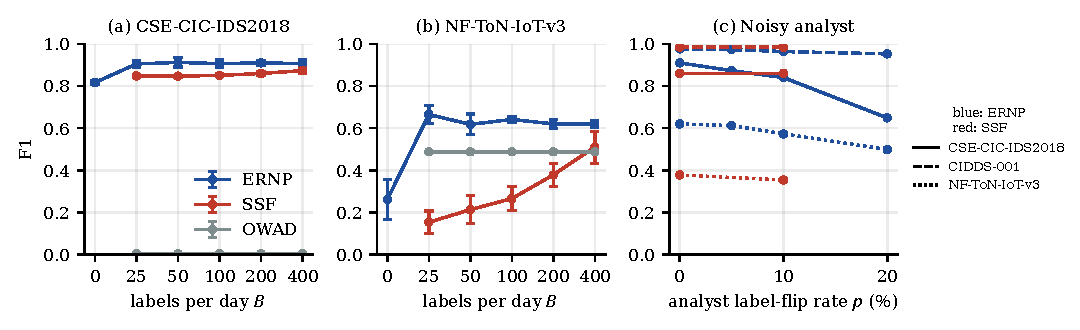
\includegraphics[width=0.98\textwidth]{fig_budget_noise.pdf}
\caption{(a,b) RQ3: F1 against the daily label budget (seeds 0--2, mean$\pm$std); OWAD detects almost nothing on CSE-CIC-IDS2018 at any budget. (c) RQ5: F1 when each returned label is flipped with probability $p$ (blue: \ERNP; red: SSF, run at $p=10\%$).}
\label{fig:budget}
\end{figure*}

\subsection{RQ4: ablations and properties}
\label{sec:rq4}
Table~\ref{tab:rq4} reports F1 differences from \ERNP. The novelty prior is the dominant component. Removing it (GBM+AL), or replacing it by Sipple's uniform prior or by a product of marginals, costs 0.26--0.29 F1 on average and up to 0.76 on CSE-CIC-IDS2018. The retraction kernel is secondary: its shape matters little (hard ball: $-0.001$), and removing retraction costs 0.017 on average and 0.093 on CSE-CIC-IDS2018. The \emph{source} of the evidence, by contrast, is decisive: the self-evidence counterfactual loses 0.50 on ToN, and it suffers the payload collapse seen in RQ2. What matters is which evidence retracts the prior, not the kernel that retracts it. ToN is the exception: GBM+AL and the other prior variants are slightly better there, because its benign traffic changes regime every day (Section~\ref{sec:discussion}).

\begin{table*}[t]
\centering
\caption{RQ4: $\Delta$F1 of each variant relative to \ERNP (five seeds).}
\label{tab:rq4}
\scriptsize
\begin{tabular}{lccccc}
\toprule
Variant ($\Delta$F1 vs. ERNP) & CIDDS-001 & NF-ToN-IoT-v3 & CIC-IDS2017$^\dagger$ & CSE-CIC-IDS2018 & Mean\\
\midrule
No novelty prior (GBM+AL) & -0.195 & +0.054 & -0.284 & -0.730 & -0.289\\
Uniform prior (Sipple) & -0.209 & +0.084 & -0.262 & -0.757 & -0.286\\
Product-of-marginals prior & -0.105 & +0.068 & -0.267 & -0.747 & -0.263\\
No retraction & -0.006 & +0.035 & -0.004 & -0.093 & -0.017\\
Hard retraction & -0.004 & +0.014 & -0.000 & -0.013 & -0.001\\
Representative-only evidence & -0.007 & -0.121 & +0.002 & -0.009 & -0.034\\
Per-flow features only & -0.003 & -0.285 & -0.033 & -0.025 & -0.086\\
No online labels & -0.028 & -0.345 & +0.000 & -0.098 & -0.118\\
Self-evidence (counterfactual) & -0.008 & -0.502 & +0.002 & -0.027 & -0.134\\
\bottomrule
\end{tabular}

\end{table*}

\textbf{Propositions on traffic.} Replaying the evidence sets, Figure~\ref{fig:p3} compares, for zero-day flows binned by their distance to the nearest confirmed benign evidence, the recall of \ERNP with that of \ERNP without online labels. At distances of $2\epsilon$ or more, \ERNP's recall is as high or higher on every dataset (ToN, $\ge4\epsilon$: 0.66 against 0.23), as Proposition~\ref{prop:p3} predicts. Recall drops only close to confirmed evidence, which is the local footprint of Proposition~\ref{prop:p1}(ii).

\textbf{Group labels.} One label per group propagates to about 12{,}000--100{,}000 flows per run, with 0.3--4.8\% attack flows inside groups labelled benign. With representative-only evidence (the label semantics of SSF), \ERNP loses 0.034 F1 on average, mostly on ToN, and remains first on average.

\begin{figure*}[t]
\centering
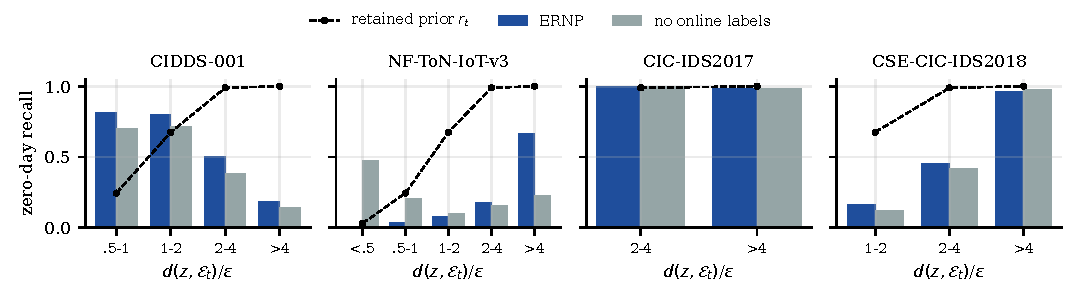
\includegraphics[width=0.98\textwidth]{fig_p3_distance.pdf}
\caption{Zero-day recall versus distance to the nearest confirmed benign evidence, in units of $\epsilon$ (bins with at least five flows; mean over five seeds). Far from evidence, \ERNP keeps at least the recall of the same detector without online labels, as Proposition~\ref{prop:p3} predicts; the dashed line is the retained prior fraction $r_t$ at the bin centre.}
\label{fig:p3}
\end{figure*}

\subsection{RQ5: sensitivity, analyst errors and cost}
\label{sec:rq5}
One-at-a-time variations of $\rho$, prior mass $m$ and bandwidth $\epsilon$ (Table~\ref{tab:rq5}) change F1 by at most 0.014 on CIDDS-001 and CSE-CIC-IDS2018. The one exception is halving $\epsilon$, which costs 0.047 on CSE-CIC-IDS2018. ToN is more sensitive (up to $+0.038$). All defaults were fixed before the evaluation and not tuned on these streams. Replacing gradient boosting by a random forest costs 0.26 on ToN, which indicates that classifier calibration matters where drift is strong.

\begin{table}[t]
\centering
\caption{RQ5: $\Delta$F1 relative to the default configuration (seeds 0--2).}
\label{tab:rq5}
\scriptsize
\setlength{\tabcolsep}{3pt}
\begin{tabular}{lccc}
\toprule
Setting ($\Delta$F1 vs. default) & CIDDS-001 & NF-ToN-IoT-v3 & CSE-CIC-IDS2018\\
\midrule
$\rho=0.1$ & +0.001 & +0.034 & +0.001\\
$\rho=0.2$ & -0.001 & +0.014 & -0.001\\
$\rho=0.5$ & -0.001 & -0.017 & +0.013\\
$m=0.25$ & -0.004 & +0.013 & -0.014\\
$m=0.5$ & -0.004 & +0.013 & -0.003\\
$m=2$ & -0.004 & +0.038 & +0.000\\
$\epsilon\times0.5$ & -0.004 & +0.007 & -0.047\\
$\epsilon\times2$ & +0.003 & +0.009 & +0.013\\
RF instead of GBM & -0.002 & -0.255 & -0.001\\
\bottomrule
\end{tabular}

\end{table}

\textbf{Analyst errors.} Proposition~\ref{prop:p1}(iii) predicts that analyst errors corrupt \ERNP locally. Figure~\ref{fig:budget}(c) flips each returned label with probability $p$:
\begin{itemize}
  \item \ERNP is robust on CIDDS-001 and CIC-IDS2017 ($-0.024$ and $-0.004$ F1 at $p=20\%$).
  \item It degrades on CSE-CIC-IDS2018 (0.910$\rightarrow$0.840 at $p=10\%$, below SSF's 0.861) and on ToN.
  \item SSF is nearly insensitive, because its labels only re-weight a supervised classifier. In \ERNP, a wrong benign label retracts the prior over an entire alert group.
\end{itemize}
In the poisoning scenario at $p=10\%$, \ERNP's zero-day payload recall still matches SSF's (0.70--0.74 against 0.67--0.72). Label noise is \ERNP's main weakness.

\textbf{Cost.} \ERNP's initial training takes 37\,s on average, against 1{,}722\,s for SSF and 709\,s for CADE. It uses the least memory and needs no GPU (Table~\ref{tab:scale}).

%======================================================================
\section{Discussion}
\label{sec:discussion}
%======================================================================
\subsection{How the five RQs form one argument}
RQ1 establishes that a detector which contrasts benign evidence with a structured prior of novelty ranks and thresholds unseen families better, on average, than detectors that model normality or known classes alone. RQ4 attributes this to the prior. RQ2 and RQ3 then show that the way the prior is adapted matters as much as the prior itself. Retraction driven only by analyst-confirmed groups keeps zero-day recall under poisoning at a budget where a continual learner loses it, and it needs about an eighth of that learner's labels. The self-evidence counterfactual closes the argument: the same model fed its own verdicts collapses.

\subsection{When ERNP does not win}
Three settings favour other methods, and we report them rather than tune \ERNP to them.
\begin{itemize}
  \item \textbf{Stable benign traffic with a strong supervised signal (CIDDS-001).} SSF's F1 is higher (0.985 vs.\ 0.976), but \ERNP ranks at least as well and recalls more attacks (Table~\ref{tab:rank}). The difference is the operating point: 0.47\% against 0.10\% FPR.
  \item \textbf{Daily regime changes of benign traffic (ToN).} Under a daily causal protocol, \ERNP's FPR reaches 42\%, and OWAD ranks ToN better. We traced this on the development seeds (0--1) with three diagnostics, all released with the code.
  \begin{enumerate}
    \item The false positives are concentrated on days on which no evidence could exist yet. On the last stream day, benign traffic moves to a new regime: \ERNP alerts on 96\% of that day's benign flows, and 96\% of those false positives carry at least one feature value seen neither in the anchor's benign traffic nor in the benign alerts of earlier days. The remaining false positives are mostly new \emph{combinations} of values that each have been confirmed before.
    \item The anchor period does not anticipate this drift. We split the anchor's benign traffic in time and trained on the first half. The flows of the second half that this model flags cover 0\% of the false positives of the first two stream days, within $2\epsilon$. Their per-feature displacement profile has cosine similarity 0.38 with that of the stream false positives, against 0.60 with that of the zero-day attacks. Transferring the anchor's drift directions would therefore retract the prior towards attacks.
    \item Removing the novelty prior (GBM+AL, five seeds) lowers the ToN FPR to 3.0\%, but raises it to 11--41\% on the other three datasets (Table~\ref{tab:rq1}).
  \end{enumerate}
  No evidence available before these days separates the new benign regime from novel attacks. A detector that must stay robust to poisoning cannot fix this with a better use of the same labels; it needs the labels sooner. With the same 200 labels per day delivered every 4\,h, \ERNP has the best F1 and MCC on ToN of all methods at that cadence (Table~\ref{tab:cadence}). The update period is therefore a deployment parameter that should follow the triage cycle.
  \item \textbf{Full scale (CIC-IDS2017).} \ERNP and CADE are on par.
\end{itemize}
We also tested four modifications of \ERNP aimed at these cases on the development seeds only: a per-feature novelty channel, a retraction kernel shaped by the observed drift, a tighter operating point, and perfectly pure alert groups (an oracle bound). None improved all datasets at once, so none was adopted.

\subsection{Operational interpretation}
\ERNP turns routine alert triage into the only adaptation signal, at the cost of a CPU refit per period. Its failure mode is explicit: an analyst who whitelists a malicious alert group whitelists its neighbourhood. The security-critical input therefore becomes the correctness of the triage decision rather than the volume of traffic, and that is where SOCs already concentrate review. In deployment, benign confirmations of large groups can be sampled for second review, and \ERNP's footprint bound (Proposition~\ref{prop:p1}(iii)) states what such a review protects.

%======================================================================
\section{Limitations and threats to validity}
\label{sec:limitations}
%======================================================================
\begin{itemize}
  \item \textbf{Update cadence.} Under daily updates, \ERNP loses on ToN to OWAD in score quality and MCC. It wins there only when labels arrive every 4\,h or faster. The cadence study uses three seeds.
  \item \textbf{Sampling.} The main results use samples of the original data. The unsampled check covers one dataset, and there CADE and SSF are stronger than on the samples.
  \item \textbf{External validity.} All four datasets come from testbeds or controlled environments, and the benign traffic of CIDDS-001 is script-generated. Results should be replicated on production traffic.
  \item \textbf{Poisoning model.} RQ2 interpolates feature vectors and is a stress test of the adaptation channel, not an end-to-end attack on a protocol stack.
  \item \textbf{Label model.} Group labels are an assumption about SOC triage. Representative-only evidence and label noise are reported, and noise at or above 10\% degrades \ERNP more than SSF.
  \item \textbf{Theory.} The propositions describe the population detector; the finite-sample classifier and the sliding evidence windows approximate it. Proposition~\ref{prop:p3} needs benign evidence to be added away from the flow in question.
  \item \textbf{Baseline deviations.} SSF's per-window epochs, Trident's percentile fallback, MemStream's normalisation variant and our port of CADE are disclosed in Table~\ref{tab:baselines}. Part of RQ2/RQ3 ran on a second machine; re-running two of those jobs locally changed F1 by at most 0.003.
  \item \textbf{Statistical power.} Four datasets give low power at the dataset level. Claims rest on per-dataset effect sizes with intervals, and the Friedman test is reported although it is not significant.
\end{itemize}

%======================================================================
\section{Conclusion}
\label{sec:conclusion}
%======================================================================
We proposed \ERNP, a NIDS that adapts only by retracting a structured novelty prior where analysts have confirmed benign traffic. The design makes the detector invariant to unlabelled traffic, ties every adaptation step to a labelled alert group, and preserves detection away from confirmed evidence. On four temporally split benchmarks, \ERNP has the best average detection against five recent detectors, including when each is run at its best configuration. It needs about an eighth of the labels of the strongest continual learner, and a counterfactual shows that its robustness to slow poisoning comes from the trusted-evidence rule. It is on par with the best baseline at full scale, and it is more sensitive than a supervised continual learner to analyst errors. Future work should make retraction robust to such errors, evaluate on operational traffic at full scale, and match the update period to the triage cycle.

\section*{CRediT authorship contribution statement}
\textbf{An Vo Le Thien:} Conceptualization, Methodology, Software, Investigation, Data curation, Formal analysis, Validation, Visualization, Writing -- original draft, Writing -- review \& editing.
% TODO(authors): add the contributions of every co-author.

\section*{Declaration of competing interest}
The authors declare that they have no known competing financial interests or personal relationships that could have appeared to influence the work reported in this paper.

\section*{Data and code availability}
The four datasets are publicly available and remain subject to the licences of their original providers. The prepared streams, the implementation of \ERNP, the wrappers around the official baseline code, the per-run predictions, and the scripts that regenerate every table and figure of this paper from those predictions are available at \url{https://github.com/volethienan/Openset_CN} (made public upon publication; available to reviewers on request). No number in the tables is typed by hand: \texttt{paper/make\_tables.py} and \texttt{paper/make\_figures.py} regenerate them from the stored evaluation records.

\section*{Declaration of generative AI and AI-assisted technologies in the manuscript preparation process}
During the preparation of this work the authors used Claude (Anthropic) in order to assist with experiment implementation, analysis scripts and language editing. After using this tool, the authors reviewed and edited the content as needed and take full responsibility for the content of the published article.

\appendix
\section{Proofs}
\label{app:proofs}
Let $b_t,a_t$ be the densities of the benign and attack evidence at period $t$, $q_0$ the initial prior and $r_t$ the retention of Eq.~\eqref{eq:retain}. Minimising $\tfrac12 b_t\,\ell(\eta,0)+\tfrac12(a_t+q_0r_t)\,\ell(\eta,1)$ pointwise over $\eta\in[0,1]$ gives the posterior behind Eq.~\eqref{eq:score}; a common positive rescaling of the weights, as used in the implementation, leaves it unchanged.

\begin{proof}[Proof of Proposition~\ref{prop:p1}]
(i) By Algorithm~\ref{alg:ernp}, $P_{t+1},A_{t+1},\E_{t+1}$ arise from $P_t,A_t,\E_t$ only by adding labelled groups, and $q_0$ and $\tau$ are fixed. Hence $s_t$ is a function of the labelled history only. Without labels, $(P_t,A_t,\E_t)=(P_0,A_0,\emptyset)$ and $s_t=s_0$.

(ii) We have $1-r_t(x)=\exp(-d(x,\E_t)^2/2\epsilon^2)>\delta$ if and only if $d(x,\E_t)<\epsilon\sqrt{2\ln(1/\delta)}=:\rho_\delta$, that is, if and only if $x$ lies in some ball $\mathcal B(e,\rho_\delta)$ with $e\in\E_t$.

(iii) Write $\E_t=\E^{c}\cup\E^{e}$, where $\E^{e}$ is the union of the $m$ erroneous groups $G_1,\dots,G_m$. Since $d(x,\E_t)=\min\{d(x,\E^c),d(x,\E^e)\}$, the errors reduce the retention at $x$ only if $d(x,\E^e)<d(x,\E^c)$. They reduce it by more than $\delta$ only if, in addition, $d(x,\E^e)<\rho_\delta$, i.e.\ $x\in\mathcal B(e,\rho_\delta)$ for some $e\in G_i$. Each $G_i$ has diameter at most $\Delta$, so $\mathcal B(e,\rho_\delta)\subseteq\mathcal B(c_i,\Delta+\rho_\delta)$ for any fixed $c_i\in G_i$. Erroneous groups enter $b_t$ only through the same $m$ labelled groups.
\end{proof}

\begin{proof}[Proof of Proposition~\ref{prop:p2}]
Since $1-e^{-u}\le u$, $r_t(x)\le d(x,\E_t)^2/(2\epsilon^2)$; the bound follows from the monotonicity of the logarithm in Eq.~\eqref{eq:score}. As $d(x,\E_t)\to0$, the bound tends to $\log(a_t(x)/b_t(x))<\tau$ under the stated condition.
\end{proof}

\begin{proof}[Proof of Proposition~\ref{prop:p3}]
Since $a_t\ge0$, $s_t(z)\ge\log(q_0(z)r_t(z))-\log b_t(z)$. The assumption $d(z,\E_t)\ge c\epsilon$ gives $r_t(z)\ge1-e^{-c^2/2}$, and $b_t(z)\le b_0(z)$ gives $-\log b_t(z)\ge-\log b_0(z)$. The margins follow from $-\log(1-e^{-2})\approx0.145$ and $-\log(1-e^{-4.5})\approx0.011$.
\end{proof}

\begin{remark}
The assumption $b_t(z)\le b_0(z)$ holds, for instance, when the benign evidence is a mixture $b_t=\lambda_t b_0+(1-\lambda_t)b_{\E}$ with $\lambda_t\le1$ and $b_{\E}(z)=0$, i.e.\ when the added benign groups lie away from $z$.
\end{remark}

\bibliographystyle{cas-model2-names}
\bibliography{refs}

\end{document}
